%  !TeX  root  =  user_guide.tex

\section{Offline Bearbeitung}\label{sec:offlinedit}

% when the revision of a section has been finalized, 
% comment out the following line:
% \updatedisclaimer

Bei der Datenerfassung ist es eine allt�gliche Situation, um mit einem 
Laptop oder Smartphone im Gel�nde offline zu arbeiten. Nach der R�ckkehr 
m�ssen die �nderungen wieder mit der Master-Datenquelle, z.B. einer PostGIS 
Datenbank synchronisiert werden. Wenn mehrere Personen gleichzeitig mit 
denselben Datenbest�nden arbeiten, ist es meist schwierig, die �nderungen 
von Hand zu verschmelzen, selbst wenn unterschiedliche Objekte ver�ndert 
wurden.

Die Erweiterung \toolbtntwo{offline_editing_copy}{Offline Bearbeitung} 
automatisiert die Synchronisation durch Kopieren des Inhalts einer 
Datenquelle (in der Regel PostGIS oder WFS-T) zu einer SpatiaLite Datenbank mit dedizierten Tabellen. Nachdem man wieder mit dem Netzwerk verbunden ist, 
k�nnen die Offline-�nderungen wieder an die Master-Datenquell zur�ckgespielt 
werden.

\minisec{Verwendung der Erweiterung}

\begin{itemize}
\item Laden Sie ein paar Vektorlayer, z.B. aus PostGIS oder WFS-T Datenquellen.
\item Speichern Sie die Einstellungen als Projekt.
\item �ffnen Sie den Dialog 'Offline Projekt erzeugen' und w�hlen Sie die Layer 
aus, die gespeichert werden sollen. Sie werden in SpatiaLite Tabellen abgelegt.
\item Editieren Sie die Layers offline.
\item Nachdem Sie wieder mit dem Internet verbunden sind, laden Sie die �nderungen wieder zur�ck, in dem Sie den 'Synchronisieren' Knopf dr�cken.
\end{itemize}

\begin{figure}[ht]
   \centering
   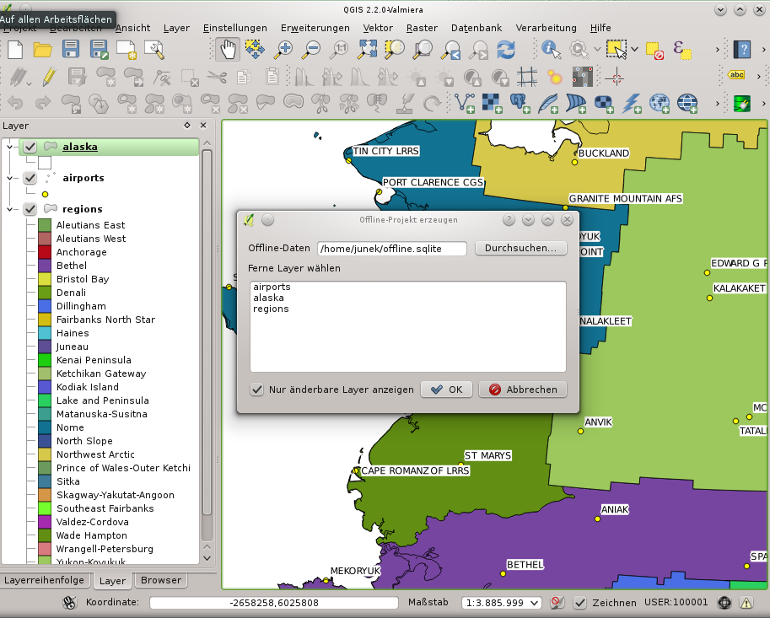
\includegraphics[clip=true, width=12cm]{create_offline_project}   
   \caption{Erstellen eines Offline-Projektes mit PostGIS Daten \nixcaption}
   \label{fig:offlineproject}
\end{figure}

\FloatBarrier
